\section{Conclusões}

Os resultados de um estudo comparativo envolvendo os pacotes $ PSOPT $, $ FALCON $ e $ COPILOTS $ foram apresentados. Discutiu-se a respeito dos estudos de caso e das métricas que devem servir de base para a implementação de um estudo comparativo adequada, e determinou-se um conjunto de estudos de caso consideravelmente heterogêneo, composto em sua maioria por problemas reais de Engenharia. Além disso, apresentaram-se os fundamentos teóricos necessários ao entendimento dos métodos empregados por cada um dos pacotes avaliados, que envolvem conceitos a respeito do Controle Ótimo e dos Métodos Diretos. 

Introduziu-se o $ COPILOTS $, pacote de código aberto para solução de PCOs desenvolvido pelo autor com base na observação das qualidades e deficiências associadas a diversos outros pacotes reportados na literatura. As principais características do $ COPILOTS $ são a simplicidade e a geração automática dos \textit{scripts} utilizados na implementação dos PCOs. Foi apresentada uma visão geral sobre as funcionalidades do pacote e sua utilização, e o mesmo foi empregado na resolução dos estudo de caso abordados no decorrer do presente trabalho. A comparação entre os resultados obtidos por meio do $ COPILOTS $ e aqueles advindos do emprego do $ PSOPT $ e do $ FALCON $ evidencia a qualidade das soluções associadas ao $ COPILOTS $.
 
Foram apresentados não só os resultados obtidos a partir do emprego de cada um dos pacotes avaliados na resolução dos estudos de caso em análise, mas também um exame detalhado acerca dos mesmos, destacando-se as principais qualidades e deficiências de cada pacote. De forma geral, recomenda-se que problemas multifásicos sejam resolvidos empregando-se o $ PSOPT $, ao mesmo tempo em que desaconselha-se a utilização desse pacote na resolução de PCOs singulares. Recomenda-se que o $ FALCON $ seja utilizado se for necessário minimizar ao máximo o tempo de processamento e o número de avaliações da função objetivo. 

Sugere-se, por fim, que o $ COPILOTS $ seja utilizado por usuários iniciantes, que tenham pouca experiência na resolução de PCOs, levando-se em conta a forma simples, direta, e sucinta com base na qual os PCOs podem ser implementados, tendo em vista que os \textit{scripts} empregados nessa tarefa são gerados e parcialmente preenchidos de forma automática, e considerando-se a sintaxe com base na qual é desenvolvido, que se assemelha consideravelmente à formulação de Bolza. Além disso, verificou-se que a implementação da colocação pseudo-espetral possibilita a obtenção de trajetórias suaves, ao passo que os melhores índices de desempenho normalmente são atribuídos às soluções obtidas por meio da colocação Hermite-Simpson. 

\section{Trabalhos futuros}

Diante dos resultados obtidos e das metodologias empregadas no desenvolvimento do presente trabalho, são apresentadas a seguir algumas propostas de melhoria a serem consideradas no desenvolvimento de trabalhos futuros. 

Primeiramente, propõe-se a utilização de métricas alternativas às utilizadas no presente trabalho, como o erro de transcrição $ \epsilon(t) $, atribuído à resolução das restrições diferenciais associadas à dinâmica do PCO. O cálculo de $ \epsilon(t) $, é baseado nas trajetórias contínuas associadas a $ \mathbf{x}(t) $ e $ \mathbf{u}(t) $, construídas a partir da interpolação dos valores assumidos por $ \mathbf{x}(t) $ e $ \mathbf{u}(t) $ nos nós de colocação. Com base nessas trajetórias e nas equações dinâmicas associadas ao PCO, computa-se $ \epsilon(t) $ segundo \eqref{eq:conclusoes:erro}. 

Com base no erro de transcrição $ \epsilon(t) $, seria possível verificar como cada um dos pacotes avaliados se comporta perante uma estratégia de refinamento de malha. Alguns pacotes como o $ PSOPT $ já dispõe de ferramentas voltadas a esse tipo de refinamento, e seria pertinente que trabalhos futuros avaliassem a eficácia dessas ferramentas perante outras abordagens e levando-se em conta o emprego de outros pacotes que dispõe de ferramentas semelhantes. 
%
\begin{equation}
	\label{eq:conclusoes:erro}
	\epsilon(t) = \mathbf{\dot{x}}(t) - \mathbf{f}(\mathbf{x}(t), \mathbf{u}(t), t)
\end{equation}

Vale ressaltar que para que seja possível utilizar métricas mais complexas, baseadas na análise de perfis de desempenho por exemplo \cite{dolan_benchmarking_2002}, é necessário que um conjunto de estudos de caso mais extenso seja proposto.

Nota-se que, dentre as métricas propostas para realização do estudo comparativo apresentado no presente trabalho, somente avaliando-se o valor ótimo da função objetivo $ J^* $ é possível dizer algo a respeito das trajetórias de controle e estado obtidas, sendo as demais métricas associadas ao processo de obtenção da solução, como por exemplo o tempo de execução $ t_p $. No entanto, a qualidade da solução não é ditada apenas por $ J^* $, o que pode ser concluído pela comparação das trajetórias de controle representadas na Figura \ref{fig:conclusoes:trajetoriasOscilatorias}, advindas da resolução do estudo de caso introduzido na Seção \ref{sec:resultados:singular1}. Nota-se a partir do emprego do $ PSOPT_l $ obtém-se um perfil de controle consideravelmente mais oscilatório que aquele advindo da utilização do $ FALCON $. No entanto, verifica-se que os $ J^* $ atribuídos a ambos os perfis são extremamente próximos, iguais a 0,26846 e 0,26851 respectivamente. Diante desse exemplo, fica clara a necessidade de se propor métricas além de $ J^* $, que possibilitem que a suavidade da trajetória seja considerada, uma vez que trajetórias de controle demasiadamente oscilatórias, que normalmente levam ao desgaste dos atuadores do sistema \cite{livne_effects_2010}, não devem ser aplicadas a sistemas reais. 

\noindent	
\begin{minipage}{\textwidth}
	\vspace{\onelineskip}
	\centering
	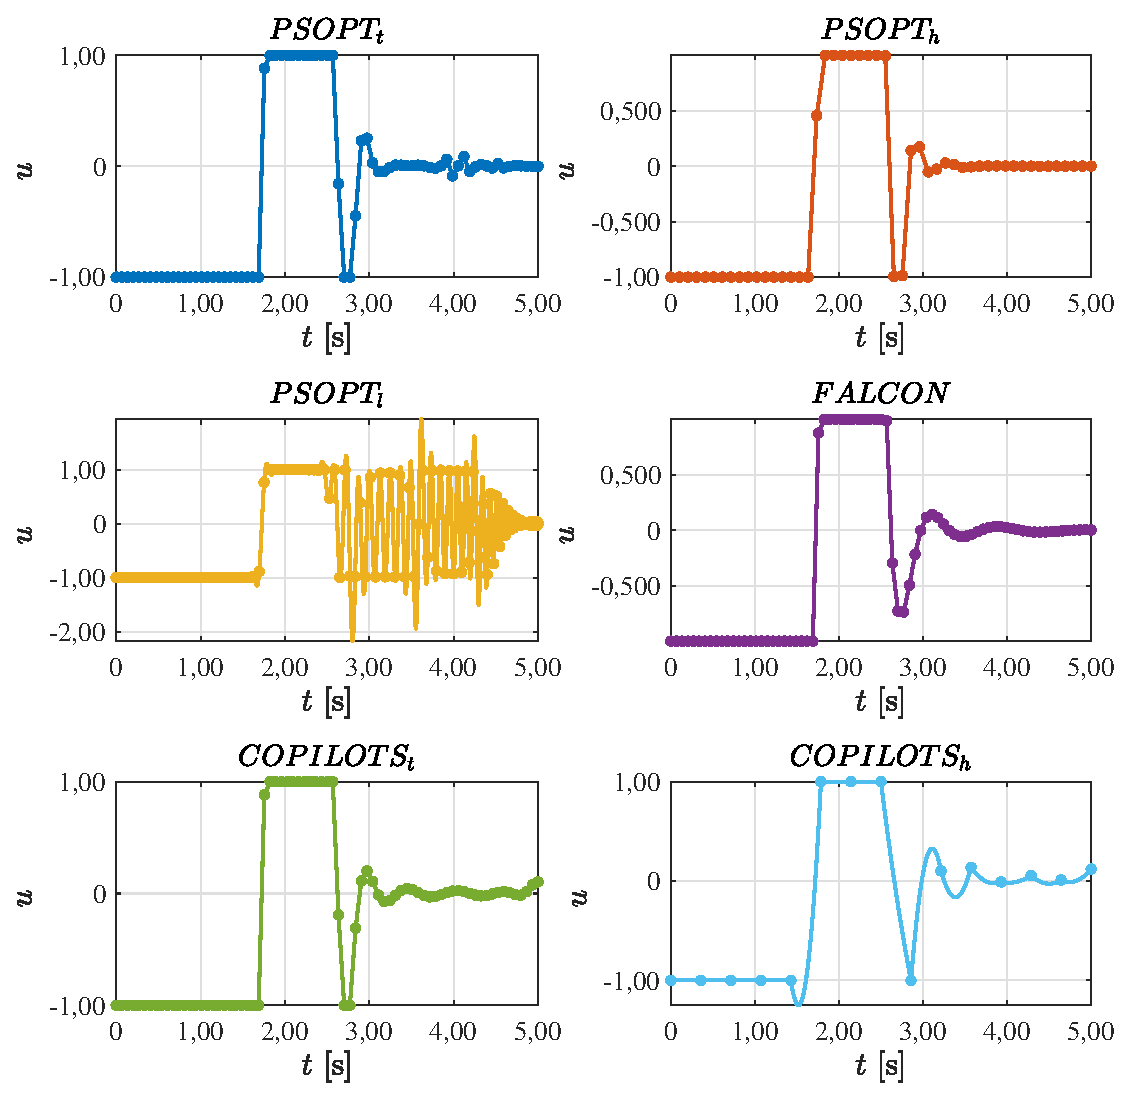
\includegraphics[width=1\linewidth]{fig/conclusoes/u}
	\captionof{figure}[Trajetórias de controle advindas da resolução do problema singular 1 a partir do emprego do $ PSOPT_l $ e do $ FALCON $]{Trajetórias de controle advindas da resolução do estudo de caso introduzido na Seção \ref{sec:resultados:singular1} a partir do emprego do $ PSOPT_l $ e do $ FALCON $.}
	\label{fig:conclusoes:trajetoriasOscilatorias}
	\vspace{\onelineskip}
\end{minipage}

Considerando que dentre os estudos de caso abordados, apenas aquele apresentado na Seção \ref{sec:resultados:foguete} é formulado empregando-se múltiplas fases, seria pertinente que outros PCOs multifásicos fossem avaliados. Os próprios PCOs singulares introduzidos na Seção \ref{sec:resultados:singulares} podem ser reformulados como PCOs multifásicos visando a obtenção de soluções mais suaves que aquelas apresentadas no presente trabalho e que estivessem associadas a $ J^* $ menores. Além disso, poderia-se atribuir a cada fase um $ N_m $ distinto, de forma a minimizar-se o número total de nós de colocação. 

Por fim, sugere-se que trabalhos futuros considerem métodos ainda não abordados de que dispõe os pacotes avaliados, como a colocação pseudo-espectral de Chebychev ou o método de Euler, associados respectivamente ao $ PSOPT $ e ao $ FALCON $.

\subsection{Melhorias a serem implementadas no $ COPILOTS $}

Apesar da qualidade dos resultados obtidos por meio do $ COPILOTS $, há espaço para implementação de diversas melhorias que devem ser incorporadas em futuras versões desse pacote. Algumas dessas melhorias, que se encontram listadas, visam possibilitar que:
%
\begin{itemize}
	\item seja utilizada a colocação pseudo-espectral;
	\item PCOs multifásicos sejam resolvidos;
	\item a implementação dos PCOs seja realizada a partir de uma interface gráfica;
	\item malhas não uniformes, com nós de colocação que não estejam igualmente espaçados no domínio do tempo, sejam implementadas;
	\item as variáveis de projeto sejam escaladas, assim como fazem o $ PSOPT $ e o $ FALCON $, no intuito de garantir que o processo de resolução dos PPNLs convirja mais rapidamente e conduza a resultados satisfatórios; 
	\item parâmetros genéricos sejam empregados na formulação dos PCOs, como fazem o $ PSOPT $ e o $ FALCON $, de forma que o $ COPILOTS $ possa ser utilizado na resolução de problemas de estimação de parâmetros e problemas inversos \cite{tarantola_inverse_2005}; 
	\item o refinamento de malha automático, baseado na verificação do erro de transcrição $ \epsilon(t) $, seja implementado;
	\item outros pacotes sejam empregados na solução dos PPNLs, como o IPOPT \cite{wachter_implementation_2006} por exemplo, utilizado pelo $ PSOPT $ e pelo $ FALCON $, visto a utilização da função \texttt{fmincon} é desencorajada pelos desenvolvedores de alguns pacotes como o ICLOCS \cite{falugi_iclocs2_2018};
	\item as funções Matlab\textsuperscript{\textregistered} utilizadas na definição das restrições e da função objetivo, sejam convertidas em arquivos \texttt{.mex}, como é feito no caso do $ FALCON $, para que o desempenho do $ COPILOTS $ seja aperfeiçoado. 
	\item o pacote \textit{Symbolic Math} \cite{mathworks_symbolic_2016} seja utilizado na computação das derivadas analíticas da função objetivo e das restrições, assim como é feito no caso do $ FALCON $, o que possibilita que os PPNLs sejam resolvidos mais rapidamente empregando um número menor de avaliações da função objetivo \cite{betts_practical_2001}. 
\end{itemize}


